% Options for packages loaded elsewhere
\PassOptionsToPackage{unicode}{hyperref}
\PassOptionsToPackage{hyphens}{url}
%
\documentclass[
]{article}
\usepackage{lmodern}
\usepackage{amssymb,amsmath}
\usepackage{ifxetex,ifluatex}
\ifnum 0\ifxetex 1\fi\ifluatex 1\fi=0 % if pdftex
  \usepackage[T1]{fontenc}
  \usepackage[utf8]{inputenc}
  \usepackage{textcomp} % provide euro and other symbols
\else % if luatex or xetex
  \usepackage{unicode-math}
  \defaultfontfeatures{Scale=MatchLowercase}
  \defaultfontfeatures[\rmfamily]{Ligatures=TeX,Scale=1}
\fi
% Use upquote if available, for straight quotes in verbatim environments
\IfFileExists{upquote.sty}{\usepackage{upquote}}{}
\IfFileExists{microtype.sty}{% use microtype if available
  \usepackage[]{microtype}
  \UseMicrotypeSet[protrusion]{basicmath} % disable protrusion for tt fonts
}{}
\makeatletter
\@ifundefined{KOMAClassName}{% if non-KOMA class
  \IfFileExists{parskip.sty}{%
    \usepackage{parskip}
  }{% else
    \setlength{\parindent}{0pt}
    \setlength{\parskip}{6pt plus 2pt minus 1pt}}
}{% if KOMA class
  \KOMAoptions{parskip=half}}
\makeatother
\usepackage{xcolor}
\IfFileExists{xurl.sty}{\usepackage{xurl}}{} % add URL line breaks if available
\IfFileExists{bookmark.sty}{\usepackage{bookmark}}{\usepackage{hyperref}}
\hypersetup{
  pdftitle={Lab2},
  pdfauthor={Irimie Fabio},
  hidelinks,
  pdfcreator={LaTeX via pandoc}}
\urlstyle{same} % disable monospaced font for URLs
\usepackage[margin=1in]{geometry}
\usepackage{color}
\usepackage{fancyvrb}
\newcommand{\VerbBar}{|}
\newcommand{\VERB}{\Verb[commandchars=\\\{\}]}
\DefineVerbatimEnvironment{Highlighting}{Verbatim}{commandchars=\\\{\}}
% Add ',fontsize=\small' for more characters per line
\usepackage{framed}
\definecolor{shadecolor}{RGB}{248,248,248}
\newenvironment{Shaded}{\begin{snugshade}}{\end{snugshade}}
\newcommand{\AlertTok}[1]{\textcolor[rgb]{0.94,0.16,0.16}{#1}}
\newcommand{\AnnotationTok}[1]{\textcolor[rgb]{0.56,0.35,0.01}{\textbf{\textit{#1}}}}
\newcommand{\AttributeTok}[1]{\textcolor[rgb]{0.77,0.63,0.00}{#1}}
\newcommand{\BaseNTok}[1]{\textcolor[rgb]{0.00,0.00,0.81}{#1}}
\newcommand{\BuiltInTok}[1]{#1}
\newcommand{\CharTok}[1]{\textcolor[rgb]{0.31,0.60,0.02}{#1}}
\newcommand{\CommentTok}[1]{\textcolor[rgb]{0.56,0.35,0.01}{\textit{#1}}}
\newcommand{\CommentVarTok}[1]{\textcolor[rgb]{0.56,0.35,0.01}{\textbf{\textit{#1}}}}
\newcommand{\ConstantTok}[1]{\textcolor[rgb]{0.00,0.00,0.00}{#1}}
\newcommand{\ControlFlowTok}[1]{\textcolor[rgb]{0.13,0.29,0.53}{\textbf{#1}}}
\newcommand{\DataTypeTok}[1]{\textcolor[rgb]{0.13,0.29,0.53}{#1}}
\newcommand{\DecValTok}[1]{\textcolor[rgb]{0.00,0.00,0.81}{#1}}
\newcommand{\DocumentationTok}[1]{\textcolor[rgb]{0.56,0.35,0.01}{\textbf{\textit{#1}}}}
\newcommand{\ErrorTok}[1]{\textcolor[rgb]{0.64,0.00,0.00}{\textbf{#1}}}
\newcommand{\ExtensionTok}[1]{#1}
\newcommand{\FloatTok}[1]{\textcolor[rgb]{0.00,0.00,0.81}{#1}}
\newcommand{\FunctionTok}[1]{\textcolor[rgb]{0.00,0.00,0.00}{#1}}
\newcommand{\ImportTok}[1]{#1}
\newcommand{\InformationTok}[1]{\textcolor[rgb]{0.56,0.35,0.01}{\textbf{\textit{#1}}}}
\newcommand{\KeywordTok}[1]{\textcolor[rgb]{0.13,0.29,0.53}{\textbf{#1}}}
\newcommand{\NormalTok}[1]{#1}
\newcommand{\OperatorTok}[1]{\textcolor[rgb]{0.81,0.36,0.00}{\textbf{#1}}}
\newcommand{\OtherTok}[1]{\textcolor[rgb]{0.56,0.35,0.01}{#1}}
\newcommand{\PreprocessorTok}[1]{\textcolor[rgb]{0.56,0.35,0.01}{\textit{#1}}}
\newcommand{\RegionMarkerTok}[1]{#1}
\newcommand{\SpecialCharTok}[1]{\textcolor[rgb]{0.00,0.00,0.00}{#1}}
\newcommand{\SpecialStringTok}[1]{\textcolor[rgb]{0.31,0.60,0.02}{#1}}
\newcommand{\StringTok}[1]{\textcolor[rgb]{0.31,0.60,0.02}{#1}}
\newcommand{\VariableTok}[1]{\textcolor[rgb]{0.00,0.00,0.00}{#1}}
\newcommand{\VerbatimStringTok}[1]{\textcolor[rgb]{0.31,0.60,0.02}{#1}}
\newcommand{\WarningTok}[1]{\textcolor[rgb]{0.56,0.35,0.01}{\textbf{\textit{#1}}}}
\usepackage{graphicx}
\makeatletter
\def\maxwidth{\ifdim\Gin@nat@width>\linewidth\linewidth\else\Gin@nat@width\fi}
\def\maxheight{\ifdim\Gin@nat@height>\textheight\textheight\else\Gin@nat@height\fi}
\makeatother
% Scale images if necessary, so that they will not overflow the page
% margins by default, and it is still possible to overwrite the defaults
% using explicit options in \includegraphics[width, height, ...]{}
\setkeys{Gin}{width=\maxwidth,height=\maxheight,keepaspectratio}
% Set default figure placement to htbp
\makeatletter
\def\fps@figure{htbp}
\makeatother
\setlength{\emergencystretch}{3em} % prevent overfull lines
\providecommand{\tightlist}{%
  \setlength{\itemsep}{0pt}\setlength{\parskip}{0pt}}
\setcounter{secnumdepth}{-\maxdimen} % remove section numbering

\title{Lab2}
\usepackage{etoolbox}
\makeatletter
\providecommand{\subtitle}[1]{% add subtitle to \maketitle
  \apptocmd{\@title}{\par {\large #1 \par}}{}{}
}
\makeatother
\subtitle{Exercises}
\author{Irimie Fabio}
\date{}

\begin{document}
\maketitle

{
\setcounter{tocdepth}{2}
\tableofcontents
}
\hypertarget{exercise-1---create-a-new-mean-and-sd-function}{%
\section{Exercise 1 - Create a new mean and sd
function}\label{exercise-1---create-a-new-mean-and-sd-function}}

\hypertarget{a}{%
\subsection{A}\label{a}}

Create the Lab2 project. Use the same structure used for Lab1:

\begin{itemize}
\tightlist
\item
  scripts,
\item
  plots,
\item
  data
\end{itemize}

\hypertarget{b}{%
\subsection{B}\label{b}}

Install the palmerpenguins package, load the penguins dataset or,
alternatively, download the .RData object from moodle and import it
after placing it inside the data directory of the project (hint: use the
load() function).

\begin{Shaded}
\begin{Highlighting}[]
\KeywordTok{library}\NormalTok{(palmerpenguins)}
\KeywordTok{data}\NormalTok{(penguins)}
\end{Highlighting}
\end{Shaded}

\hypertarget{c}{%
\subsection{C}\label{c}}

Compute the mean, the standard deviation, and the median for the numeric
variables of the dataset.

\begin{Shaded}
\begin{Highlighting}[]
\CommentTok{\# Means}
\KeywordTok{cat}\NormalTok{(}\StringTok{"Means: }\CharTok{\textbackslash{}n}\StringTok{"}\NormalTok{)}
\CommentTok{\#\# Means:}
\KeywordTok{colMeans}\NormalTok{(penguins[, }\KeywordTok{c}\NormalTok{(}\DecValTok{3}\OperatorTok{:}\DecValTok{6}\NormalTok{, }\DecValTok{8}\NormalTok{)], }\DataTypeTok{na.rm =} \OtherTok{TRUE}\NormalTok{)}
\CommentTok{\#\#    bill\_length\_mm     bill\_depth\_mm flipper\_length\_mm       body\_mass\_g }
\CommentTok{\#\#          43.92193          17.15117         200.91520        4201.75439 }
\CommentTok{\#\#              year }
\CommentTok{\#\#        2008.02907}
\KeywordTok{cat}\NormalTok{(}\StringTok{"}\CharTok{\textbackslash{}n}\StringTok{"}\NormalTok{)}

\CommentTok{\# Medians}
\KeywordTok{cat}\NormalTok{(}\StringTok{"Medians: }\CharTok{\textbackslash{}n}\StringTok{"}\NormalTok{)}
\CommentTok{\#\# Medians:}
\KeywordTok{sapply}\NormalTok{(penguins[, }\KeywordTok{c}\NormalTok{(}\DecValTok{3}\OperatorTok{:}\DecValTok{6}\NormalTok{, }\DecValTok{8}\NormalTok{)], median, }\DataTypeTok{na.rm =} \OtherTok{TRUE}\NormalTok{)}
\CommentTok{\#\#    bill\_length\_mm     bill\_depth\_mm flipper\_length\_mm       body\_mass\_g }
\CommentTok{\#\#             44.45             17.30            197.00           4050.00 }
\CommentTok{\#\#              year }
\CommentTok{\#\#           2008.00}
\KeywordTok{cat}\NormalTok{(}\StringTok{"}\CharTok{\textbackslash{}n}\StringTok{"}\NormalTok{)}

\CommentTok{\# Standard deviations}
\KeywordTok{cat}\NormalTok{(}\StringTok{"Standard deviations: }\CharTok{\textbackslash{}n}\StringTok{"}\NormalTok{)}
\CommentTok{\#\# Standard deviations:}
\KeywordTok{sapply}\NormalTok{(penguins[, }\KeywordTok{c}\NormalTok{(}\DecValTok{3}\OperatorTok{:}\DecValTok{6}\NormalTok{, }\DecValTok{8}\NormalTok{)], sd, }\DataTypeTok{na.rm =} \OtherTok{TRUE}\NormalTok{)}
\CommentTok{\#\#    bill\_length\_mm     bill\_depth\_mm flipper\_length\_mm       body\_mass\_g }
\CommentTok{\#\#         5.4595837         1.9747932        14.0617137       801.9545357 }
\CommentTok{\#\#              year }
\CommentTok{\#\#         0.8183559}
\KeywordTok{cat}\NormalTok{(}\StringTok{"}\CharTok{\textbackslash{}n}\StringTok{"}\NormalTok{)}
\end{Highlighting}
\end{Shaded}

\hypertarget{d}{%
\subsection{D}\label{d}}

Create a function called stat\_auto that simultaneously returns both the
mean and the standard deviation of a given vector (hint: return an
object of type list or simply a vector). Then try it on the same numeric
variables in C. to check the results (hint: if you obtain NA maybe you
forgot to remove NA terms in the vector).

\begin{Shaded}
\begin{Highlighting}[]
\NormalTok{stat\_auto \textless{}{-}}\StringTok{ }\ControlFlowTok{function}\NormalTok{(vec, }\DataTypeTok{na.rm =} \OtherTok{FALSE}\NormalTok{) \{}
  \ControlFlowTok{if}\NormalTok{ (na.rm) \{}
\NormalTok{    mean \textless{}{-}}\StringTok{ }\KeywordTok{mean}\NormalTok{(vec, }\DataTypeTok{na.rm =} \OtherTok{TRUE}\NormalTok{)}
\NormalTok{    sd \textless{}{-}}\StringTok{ }\KeywordTok{sd}\NormalTok{(vec, }\DataTypeTok{na.rm =} \OtherTok{TRUE}\NormalTok{)}

    \KeywordTok{return}\NormalTok{(}\KeywordTok{list}\NormalTok{(}\StringTok{"mean"}\NormalTok{ =}\StringTok{ }\NormalTok{mean, }\StringTok{"sd"}\NormalTok{ =}\StringTok{ }\NormalTok{sd))}
\NormalTok{  \}}

\NormalTok{  mean \textless{}{-}}\StringTok{ }\KeywordTok{mean}\NormalTok{(vec)}
\NormalTok{  sd \textless{}{-}}\StringTok{ }\KeywordTok{sd}\NormalTok{(vec)}

  \KeywordTok{return}\NormalTok{(}\KeywordTok{list}\NormalTok{(}\StringTok{"mean"}\NormalTok{ =}\StringTok{ }\NormalTok{mean, }\StringTok{"sd"}\NormalTok{ =}\StringTok{ }\NormalTok{sd))}
\NormalTok{\}}

\KeywordTok{sapply}\NormalTok{(penguins[, }\KeywordTok{c}\NormalTok{(}\DecValTok{3}\OperatorTok{:}\DecValTok{6}\NormalTok{, }\DecValTok{8}\NormalTok{)], stat\_auto, }\DataTypeTok{na.rm =} \OtherTok{TRUE}\NormalTok{)}
\end{Highlighting}
\end{Shaded}

\begin{verbatim}
##      bill_length_mm bill_depth_mm flipper_length_mm body_mass_g
## mean 43.92193       17.15117      200.9152          4201.754   
## sd   5.459584       1.974793      14.06171          801.9545   
##      year     
## mean 2008.029 
## sd   0.8183559
\end{verbatim}

\hypertarget{e}{%
\subsection{E}\label{e}}

Create a function called stat\_manual that simultaneously returns both
the mean and the standard deviation of a given vector without using the
mean() and the sd() functions (hint: you can use length(), sum(), and
na.omit() functions). Then try it on the same numeric variables in C. to
check the results.

\begin{Shaded}
\begin{Highlighting}[]
\NormalTok{stat\_manual \textless{}{-}}\StringTok{ }\ControlFlowTok{function}\NormalTok{(vec, }\DataTypeTok{na.rm =} \OtherTok{FALSE}\NormalTok{) \{}
  \ControlFlowTok{if}\NormalTok{ (na.rm) \{}
\NormalTok{    sum \textless{}{-}}\StringTok{ }\KeywordTok{sum}\NormalTok{(vec, }\DataTypeTok{na.rm =} \OtherTok{TRUE}\NormalTok{)}
\NormalTok{    mean \textless{}{-}}\StringTok{ }\NormalTok{sum }\OperatorTok{/}\StringTok{ }\KeywordTok{na.omit}\NormalTok{(}\KeywordTok{length}\NormalTok{(vec))}

\NormalTok{    sum \textless{}{-}}\StringTok{ }\KeywordTok{sum}\NormalTok{((vec }\OperatorTok{{-}}\StringTok{ }\NormalTok{mean)}\OperatorTok{\^{}}\DecValTok{2}\NormalTok{, }\DataTypeTok{na.rm =} \OtherTok{TRUE}\NormalTok{)}
\NormalTok{    denom \textless{}{-}}\StringTok{ }\KeywordTok{na.omit}\NormalTok{(}\KeywordTok{length}\NormalTok{(vec)) }\OperatorTok{{-}}\StringTok{ }\DecValTok{1}
\NormalTok{    varianza \textless{}{-}}\StringTok{ }\NormalTok{sum }\OperatorTok{/}\StringTok{ }\NormalTok{denom}

\NormalTok{    sd \textless{}{-}}\StringTok{ }\KeywordTok{sqrt}\NormalTok{(varianza)}

    \KeywordTok{return}\NormalTok{(}\KeywordTok{list}\NormalTok{(}\StringTok{"mean"}\NormalTok{ =}\StringTok{ }\NormalTok{mean, }\StringTok{"sd"}\NormalTok{ =}\StringTok{ }\NormalTok{sd))}
\NormalTok{  \}}

\NormalTok{  sum \textless{}{-}}\StringTok{ }\KeywordTok{sum}\NormalTok{(vec)}
\NormalTok{  mean \textless{}{-}}\StringTok{ }\NormalTok{sum }\OperatorTok{/}\StringTok{ }\KeywordTok{length}\NormalTok{(vec)}

\NormalTok{  sum \textless{}{-}}\StringTok{ }\KeywordTok{sum}\NormalTok{((vec }\OperatorTok{{-}}\StringTok{ }\NormalTok{mean)}\OperatorTok{\^{}}\DecValTok{2}\NormalTok{)}
\NormalTok{  denom \textless{}{-}}\StringTok{ }\KeywordTok{length}\NormalTok{(vec) }\OperatorTok{{-}}\StringTok{ }\DecValTok{1}
\NormalTok{  varianza \textless{}{-}}\StringTok{ }\NormalTok{sum }\OperatorTok{/}\StringTok{ }\NormalTok{denom}

\NormalTok{  sd \textless{}{-}}\StringTok{ }\KeywordTok{sqrt}\NormalTok{(varianza)}

  \KeywordTok{return}\NormalTok{(}\KeywordTok{list}\NormalTok{(}\StringTok{"mean"}\NormalTok{ =}\StringTok{ }\NormalTok{mean, }\StringTok{"sd"}\NormalTok{ =}\StringTok{ }\NormalTok{sd))}
\NormalTok{\}}

\KeywordTok{sapply}\NormalTok{(penguins[, }\KeywordTok{c}\NormalTok{(}\DecValTok{3}\OperatorTok{:}\DecValTok{6}\NormalTok{, }\DecValTok{8}\NormalTok{)], stat\_manual, }\DataTypeTok{na.rm =} \OtherTok{TRUE}\NormalTok{)}
\end{Highlighting}
\end{Shaded}

\begin{verbatim}
##      bill_length_mm bill_depth_mm flipper_length_mm body_mass_g
## mean 43.66657       17.05145      199.7471          4177.326   
## sd   5.449612       1.971543      14.06909          799.985    
##      year     
## mean 2008.029 
## sd   0.8183559
\end{verbatim}

\hypertarget{exercise-2---table-of-frequencies}{%
\section{Exercise 2 - Table of
frequencies}\label{exercise-2---table-of-frequencies}}

\hypertarget{a-1}{%
\subsection{A}\label{a-1}}

In the penguins dataset, transform a numeric variable to a categorical
one by aggregating values into classes. Consider the flipper length
variable and create 10mm wide classes using the cut() function (hint:
use the range() function to determine the min and max values of the
variable, then define a sequence for the cuts).

\begin{Shaded}
\begin{Highlighting}[]
\NormalTok{r \textless{}{-}}\StringTok{ }\KeywordTok{range}\NormalTok{(penguins}\OperatorTok{$}\NormalTok{flipper\_length\_mm, }\DataTypeTok{na.rm =} \OtherTok{TRUE}\NormalTok{)}
\NormalTok{splits \textless{}{-}}\StringTok{ }\KeywordTok{seq}\NormalTok{(r[}\DecValTok{1}\NormalTok{], r[}\DecValTok{2}\NormalTok{], }\DecValTok{10}\NormalTok{)}
\NormalTok{splits \textless{}{-}}\StringTok{ }\KeywordTok{append}\NormalTok{(splits, r[}\DecValTok{2}\NormalTok{])}

\NormalTok{classes \textless{}{-}}\StringTok{ }\KeywordTok{cut}\NormalTok{(penguins}\OperatorTok{$}\NormalTok{flipper\_length\_mm, splits, }\DataTypeTok{ordered\_result =} \OtherTok{TRUE}\NormalTok{)}

\KeywordTok{cat}\NormalTok{(}\StringTok{"Splits: "}\NormalTok{, splits, }\StringTok{"}\CharTok{\textbackslash{}n}\StringTok{"}\NormalTok{)}
\end{Highlighting}
\end{Shaded}

\begin{verbatim}
## Splits:  172 182 192 202 212 222 231
\end{verbatim}

\begin{Shaded}
\begin{Highlighting}[]
\KeywordTok{cat}\NormalTok{(}\StringTok{"Classes: }\CharTok{\textbackslash{}n}\StringTok{"}\NormalTok{)}
\end{Highlighting}
\end{Shaded}

\begin{verbatim}
## Classes:
\end{verbatim}

\begin{Shaded}
\begin{Highlighting}[]
\NormalTok{classes}
\end{Highlighting}
\end{Shaded}

\begin{verbatim}
##   [1] (172,182] (182,192] (192,202] <NA>      (192,202] (182,192]
##   [7] (172,182] (192,202] (192,202] (182,192] (182,192] (172,182]
##  [13] (172,182] (182,192] (192,202] (182,192] (192,202] (192,202]
##  [19] (182,192] (192,202] (172,182] (172,182] (182,192] (182,192]
##  [25] (172,182] (182,192] (182,192] (182,192] <NA>      (172,182]
##  [31] (172,182] (172,182] (182,192] (182,192] (192,202] (192,202]
##  [37] (182,192] (172,182] (172,182] (182,192] (172,182] (192,202]
##  [43] (182,192] (192,202] (182,192] (182,192] (172,182] (172,182]
##  [49] (182,192] (182,192] (182,192] (182,192] (182,192] (192,202]
##  [55] (182,192] (182,192] (182,192] (192,202] (172,182] (192,202]
##  [61] (182,192] (192,202] (182,192] (182,192] (182,192] (182,192]
##  [67] (192,202] (182,192] (182,192] (192,202] (182,192] (182,192]
##  [73] (192,202] (192,202] (182,192] (192,202] (182,192] (182,192]
##  [79] (182,192] (192,202] (182,192] (192,202] (182,192] (192,202]
##  [85] (182,192] (192,202] (182,192] (182,192] (182,192] (182,192]
##  [91] (192,202] (202,212] (182,192] (182,192] (182,192] (202,212]
##  [97] (182,192] (192,202] (172,182] (182,192] (182,192] (202,212]
## [103] (182,192] (182,192] (192,202] (182,192] (192,202] (182,192]
## [109] (172,182] (192,202] (192,202] (182,192] (192,202] (192,202]
## [115] (182,192] (192,202] (182,192] (192,202] (182,192] (182,192]
## [121] (182,192] (192,202] (172,182] (192,202] (182,192] (192,202]
## [127] (182,192] (192,202] (182,192] (202,212] (182,192] (192,202]
## [133] (192,202] (192,202] (182,192] (182,192] (182,192] (192,202]
## [139] (182,192] (192,202] (192,202] (182,192] (182,192] (182,192]
## [145] (182,192] (182,192] (182,192] (182,192] (192,202] (192,202]
## [151] (182,192] (192,202] (202,212] (222,231] (202,212] (212,222]
## [157] (212,222] (202,212] (202,212] (212,222] (202,212] (212,222]
## [163] (212,222] (212,222] (212,222] (212,222] (202,212] (212,222]
## [169] (202,212] (212,222] (202,212] (212,222] (212,222] (212,222]
## [175] (212,222] (212,222] (212,222] (212,222] (212,222] (212,222]
## [181] (202,212] (212,222] (212,222] (202,212] (202,212] (222,231]
## [187] (212,222] (212,222] (212,222] (212,222] (202,212] (202,212]
## [193] (202,212] (222,231] (202,212] (212,222] (212,222] (212,222]
## [199] (202,212] (222,231] (212,222] (212,222] (202,212] (212,222]
## [205] (202,212] (222,231] (212,222] (212,222] (202,212] (212,222]
## [211] (202,212] (222,231] (202,212] (212,222] (212,222] (222,231]
## [217] (212,222] (222,231] (212,222] (222,231] (212,222] (222,231]
## [223] (212,222] (212,222] (212,222] (212,222] (212,222] (222,231]
## [229] (202,212] (212,222] (212,222] (222,231] (202,212] (212,222]
## [235] (202,212] (222,231] (202,212] (222,231] (212,222] (212,222]
## [241] (202,212] (222,231] (212,222] (222,231] (202,212] (222,231]
## [247] (212,222] (222,231] (212,222] (212,222] (202,212] (222,231]
## [253] (212,222] (222,231] (212,222] (222,231] (212,222] (212,222]
## [259] (202,212] (212,222] (202,212] (202,212] (212,222] (222,231]
## [265] (212,222] (222,231] (212,222] (222,231] (212,222] (212,222]
## [271] (212,222] <NA>      (212,222] (212,222] (202,212] (212,222]
## [277] (182,192] (192,202] (192,202] (182,192] (192,202] (192,202]
## [283] (172,182] (192,202] (192,202] (192,202] (192,202] (192,202]
## [289] (182,192] (192,202] (182,192] (192,202] (192,202] (172,182]
## [295] (182,192] (192,202] (172,182] (182,192] (182,192] (192,202]
## [301] (192,202] (192,202] (192,202] (192,202] (182,192] (202,212]
## [307] (182,192] (192,202] (182,192] (202,212] (192,202] (192,202]
## [313] (192,202] (202,212] (182,192] (202,212] (202,212] (182,192]
## [319] (192,202] (192,202] (192,202] (192,202] (182,192] (202,212]
## [325] (182,192] (192,202] (192,202] (192,202] (192,202] (202,212]
## [331] (182,192] (192,202] (182,192] (202,212] (192,202] (192,202]
## [337] (202,212] (182,192] (192,202] (202,212] (192,202] (192,202]
## [343] (202,212] (192,202]
## 6 Levels: (172,182] < (182,192] < (192,202] < ... < (222,231]
\end{verbatim}

\hypertarget{b-1}{%
\subsection{B}\label{b-1}}

Use the table() function on the new variable generated by cut(). Then
transform it into a data.frame object. Rename the columns accordingly
using the colnames() function (hint: the second column correspond to the
absolute frequencies).

\begin{Shaded}
\begin{Highlighting}[]
\NormalTok{df \textless{}{-}}\StringTok{ }\KeywordTok{data.frame}\NormalTok{(}\KeywordTok{table}\NormalTok{(classes))}
\KeywordTok{colnames}\NormalTok{(df) \textless{}{-}}\StringTok{ }\KeywordTok{c}\NormalTok{(}\StringTok{"Classes"}\NormalTok{, }\StringTok{"AbsoluteFrequencies"}\NormalTok{)}
\NormalTok{df}
\end{Highlighting}
\end{Shaded}

\begin{verbatim}
##     Classes AbsoluteFrequencies
## 1 (172,182]                  22
## 2 (182,192]                  96
## 3 (192,202]                  85
## 4 (202,212]                  47
## 5 (212,222]                  67
## 6 (222,231]                  24
\end{verbatim}

\hypertarget{c-1}{%
\subsection{C}\label{c-1}}

Add the the columns for: relative frequencies, cumulative absolute
frequencies, and cumulative relative frequencies.

\begin{Shaded}
\begin{Highlighting}[]
\NormalTok{df}\OperatorTok{$}\NormalTok{CumAbsFreq \textless{}{-}}\StringTok{ }\KeywordTok{cumsum}\NormalTok{(df}\OperatorTok{$}\NormalTok{AbsoluteFrequencies)}
\NormalTok{df}\OperatorTok{$}\NormalTok{RelativeFrequencies \textless{}{-}}\StringTok{ }\NormalTok{df}\OperatorTok{$}\NormalTok{AbsoluteFrequencies }\OperatorTok{/}\StringTok{ }\KeywordTok{sum}\NormalTok{(df}\OperatorTok{$}\NormalTok{AbsoluteFrequencies)}
\NormalTok{df}\OperatorTok{$}\NormalTok{RelAbsFreq \textless{}{-}}\StringTok{ }\KeywordTok{cumsum}\NormalTok{(df}\OperatorTok{$}\NormalTok{RelativeFrequencies)}
\NormalTok{df}
\end{Highlighting}
\end{Shaded}

\begin{verbatim}
##     Classes AbsoluteFrequencies CumAbsFreq RelativeFrequencies
## 1 (172,182]                  22         22          0.06451613
## 2 (182,192]                  96        118          0.28152493
## 3 (192,202]                  85        203          0.24926686
## 4 (202,212]                  47        250          0.13782991
## 5 (212,222]                  67        317          0.19648094
## 6 (222,231]                  24        341          0.07038123
##   RelAbsFreq
## 1 0.06451613
## 2 0.34604106
## 3 0.59530792
## 4 0.73313783
## 5 0.92961877
## 6 1.00000000
\end{verbatim}

\hypertarget{d-1}{%
\subsection{D}\label{d-1}}

Use the geom\_col() function to plot the frequence of each class. Then,
using the geom\_text(aes(label = \ldots)) function, add the relative
frequence as a percentage above each column (hint: substitute the
\ldots{} with the relative frequency values. Use the round() function to
choose the appropriate number of digits).

\begin{Shaded}
\begin{Highlighting}[]
\KeywordTok{library}\NormalTok{(ggplot2)}
\KeywordTok{ggplot}\NormalTok{(}
  \DataTypeTok{data =}\NormalTok{ df,}
  \KeywordTok{aes}\NormalTok{(}
    \DataTypeTok{x =}\NormalTok{ df}\OperatorTok{$}\NormalTok{Class,}
    \DataTypeTok{y =}\NormalTok{ df}\OperatorTok{$}\NormalTok{AbsoluteFrequency,}
\NormalTok{  )}
\NormalTok{) }\OperatorTok{+}
\StringTok{  }\KeywordTok{geom\_col}\NormalTok{(}\KeywordTok{aes}\NormalTok{(}\DataTypeTok{y =}\NormalTok{ df}\OperatorTok{$}\NormalTok{AbsoluteFrequencies)) }\OperatorTok{+}
\StringTok{  }\KeywordTok{geom\_text}\NormalTok{(}
    \KeywordTok{aes}\NormalTok{(}
      \DataTypeTok{label =} \KeywordTok{paste}\NormalTok{(}\KeywordTok{round}\NormalTok{(df}\OperatorTok{$}\NormalTok{RelativeFrequencies }\OperatorTok{*}\StringTok{ }\DecValTok{100}\NormalTok{, }\DecValTok{2}\NormalTok{), }\StringTok{"\%"}\NormalTok{),}
      \DataTypeTok{y =}\NormalTok{ df}\OperatorTok{$}\NormalTok{AbsoluteFrequencies,}
\NormalTok{    ),}
    \DataTypeTok{vjust =} \FloatTok{{-}0.5}\NormalTok{,}
\NormalTok{  ) }\OperatorTok{+}
\StringTok{  }\KeywordTok{labs}\NormalTok{(}
    \DataTypeTok{title =} \StringTok{"Flipper length by class"}\NormalTok{,}
    \DataTypeTok{x =} \StringTok{"Flipper length class (mm)"}\NormalTok{,}
    \DataTypeTok{y =} \StringTok{"Absolute frequency"}\NormalTok{,}
\NormalTok{  ) }\OperatorTok{+}
\StringTok{  }\KeywordTok{theme}\NormalTok{(}\DataTypeTok{legend.position =} \StringTok{"bottom"}\NormalTok{)}
\end{Highlighting}
\end{Shaded}

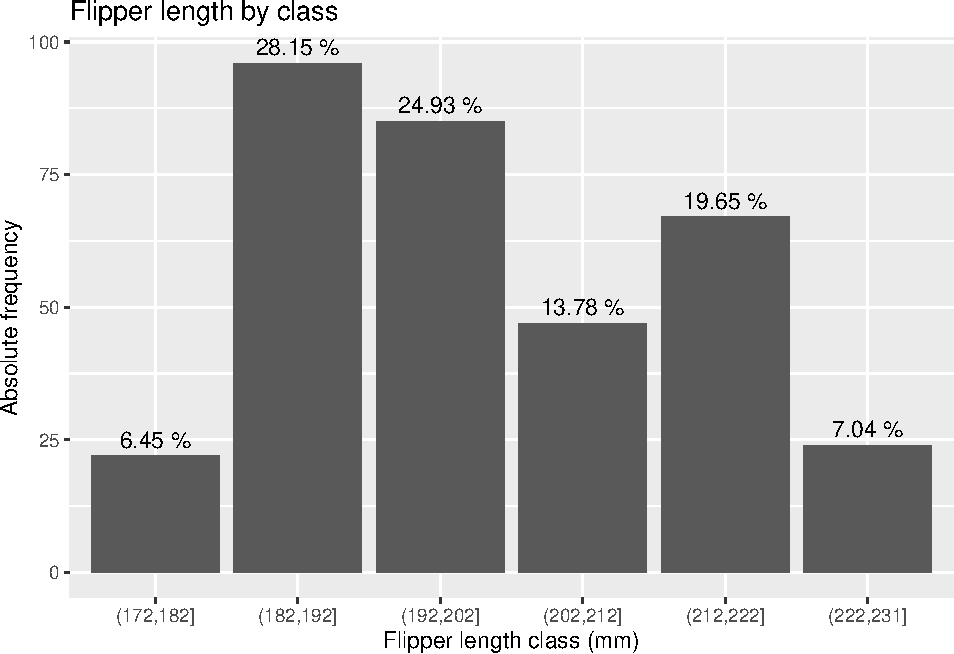
\includegraphics{es_files/figure-latex/unnamed-chunk-8-1.pdf}

\hypertarget{exercise-3---histogram-boxplot-and-quartiles}{%
\section{Exercise 3 - Histogram, Boxplot and
quartiles}\label{exercise-3---histogram-boxplot-and-quartiles}}

\hypertarget{a-2}{%
\subsection{A}\label{a-2}}

Using the geom\_histogram() function of the ggplot2 package plot the
flipper length distribution coloring each species with a different color
(hint: use the fill argument of the aes() function to fill the\\
histogram area and the position = ``identity'' argument of the
geom\_histogram()). Play with the binwidth argument. Try to insert y =
..density.. in aes(). Do you notice any change?

\begin{Shaded}
\begin{Highlighting}[]
\KeywordTok{ggplot}\NormalTok{(}
  \DataTypeTok{data =}\NormalTok{ penguins,}
  \KeywordTok{aes}\NormalTok{(}
    \DataTypeTok{x =}\NormalTok{ penguins}\OperatorTok{$}\NormalTok{flipper\_length\_mm,}
    \DataTypeTok{fill =}\NormalTok{ penguins}\OperatorTok{$}\NormalTok{species,}
\NormalTok{  )}
\NormalTok{) }\OperatorTok{+}
\StringTok{  }\KeywordTok{scale\_fill\_manual}\NormalTok{(}\DataTypeTok{values =} \KeywordTok{c}\NormalTok{(}\StringTok{"darkorange"}\NormalTok{, }\StringTok{"purple"}\NormalTok{, }\StringTok{"cyan4"}\NormalTok{)) }\OperatorTok{+}
\StringTok{  }\KeywordTok{geom\_histogram}\NormalTok{(}
    \DataTypeTok{position =} \StringTok{"identity"}\NormalTok{,}
    \DataTypeTok{binwidth =} \DecValTok{2}\NormalTok{,}
    \KeywordTok{aes}\NormalTok{(}\DataTypeTok{y =}\NormalTok{ ..density..),}
\NormalTok{  ) }\OperatorTok{+}
\StringTok{  }\KeywordTok{labs}\NormalTok{(}
    \DataTypeTok{title =} \StringTok{"Flipper length distribution"}\NormalTok{,}
    \DataTypeTok{x =} \StringTok{"Flipper length (mm)"}\NormalTok{,}
    \DataTypeTok{y =} \StringTok{"Density"}\NormalTok{,}
    \DataTypeTok{fill =} \StringTok{"Species"}\NormalTok{,}
\NormalTok{  ) }\OperatorTok{+}
\StringTok{  }\KeywordTok{theme}\NormalTok{(}\DataTypeTok{legend.position =} \StringTok{"bottom"}\NormalTok{)}
\end{Highlighting}
\end{Shaded}

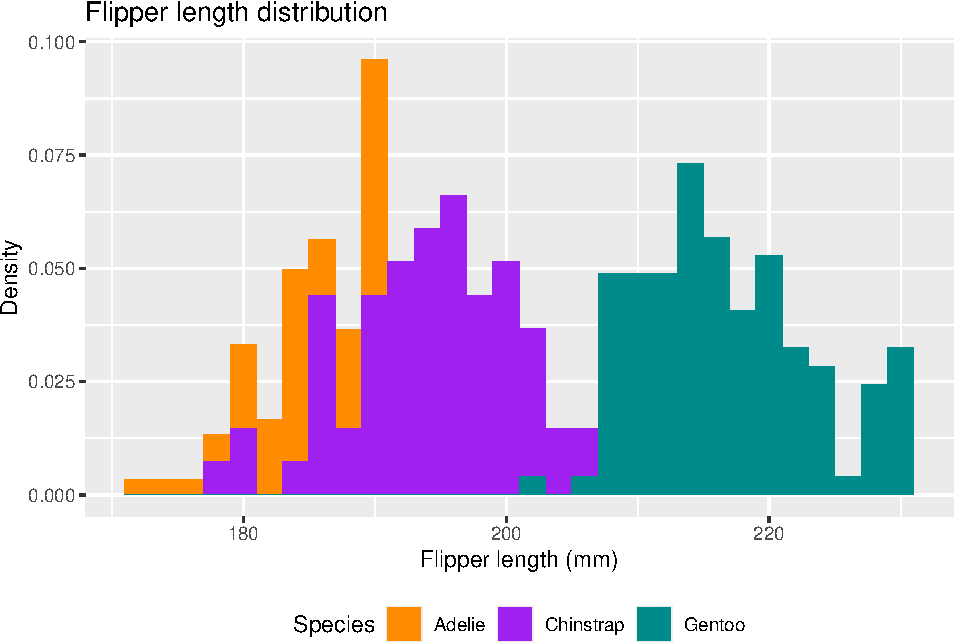
\includegraphics{es_files/figure-latex/unnamed-chunk-9-1.pdf}

\hypertarget{b-2}{%
\subsection{B}\label{b-2}}

About the flipper length, for each species of penguins compute the: 1.
Sample mean 2. Sample median 3. Sample standard deviation (use a
division by \(n-1\)) 4. Sample variance

(hint: to choose only a specific species use
penguins{[}penguins\$species == ``Gentoo'',{]})

\begin{Shaded}
\begin{Highlighting}[]
\NormalTok{species \textless{}{-}}\StringTok{ }\KeywordTok{unique}\NormalTok{(penguins}\OperatorTok{$}\NormalTok{species)}
\NormalTok{summary \textless{}{-}}\StringTok{ }\KeywordTok{data.frame}\NormalTok{(}
  \DataTypeTok{Specie =}\NormalTok{ species}
\NormalTok{)}

\ControlFlowTok{for}\NormalTok{ (specie }\ControlFlowTok{in}\NormalTok{ species) \{}
\NormalTok{  summary}\OperatorTok{$}\NormalTok{Mean[}\KeywordTok{which}\NormalTok{(specie }\OperatorTok{==}\StringTok{ }\NormalTok{species)] \textless{}{-}}
\StringTok{    }\KeywordTok{mean}\NormalTok{(penguins[penguins}\OperatorTok{$}\NormalTok{species }\OperatorTok{==}\StringTok{ }\NormalTok{specie, ]}\OperatorTok{$}\NormalTok{flipper\_length\_mm,}
      \DataTypeTok{na.rm =} \OtherTok{TRUE}
\NormalTok{    )}
\NormalTok{  summary}\OperatorTok{$}\NormalTok{Median[}\KeywordTok{which}\NormalTok{(specie }\OperatorTok{==}\StringTok{ }\NormalTok{species)] \textless{}{-}}
\StringTok{    }\KeywordTok{median}\NormalTok{(penguins[penguins}\OperatorTok{$}\NormalTok{species }\OperatorTok{==}\StringTok{ }\NormalTok{specie, ]}\OperatorTok{$}\NormalTok{flipper\_length\_mm,}
      \DataTypeTok{na.rm =} \OtherTok{TRUE}
\NormalTok{    )}
\NormalTok{  summary}\OperatorTok{$}\NormalTok{StandardDeviation[}\KeywordTok{which}\NormalTok{(specie }\OperatorTok{==}\StringTok{ }\NormalTok{species)] \textless{}{-}}
\StringTok{    }\KeywordTok{sd}\NormalTok{(penguins[penguins}\OperatorTok{$}\NormalTok{species }\OperatorTok{==}\StringTok{ }\NormalTok{specie, ]}\OperatorTok{$}\NormalTok{flipper\_length\_mm,}
      \DataTypeTok{na.rm =} \OtherTok{TRUE}
\NormalTok{    )}
\NormalTok{  summary}\OperatorTok{$}\NormalTok{Variance[}\KeywordTok{which}\NormalTok{(specie }\OperatorTok{==}\StringTok{ }\NormalTok{species)] \textless{}{-}}
\StringTok{    }\KeywordTok{var}\NormalTok{(penguins[penguins}\OperatorTok{$}\NormalTok{species }\OperatorTok{==}\StringTok{ }\NormalTok{specie, ]}\OperatorTok{$}\NormalTok{flipper\_length\_mm,}
      \DataTypeTok{na.rm =} \OtherTok{TRUE}
\NormalTok{    )}
\NormalTok{\}}
\NormalTok{summary}
\end{Highlighting}
\end{Shaded}

\begin{verbatim}
##      Specie     Mean Median StandardDeviation Variance
## 1    Adelie 189.9536    190          6.539457 42.76450
## 2    Gentoo 217.1870    216          6.484976 42.05491
## 3 Chinstrap 195.8235    196          7.131894 50.86392
\end{verbatim}

\hypertarget{c-2}{%
\subsection{C}\label{c-2}}

Using the geom\_boxplot() function of the ggplot2 package plot the
boxplot for the flipper length variable coloring each species with a
different color (hint: use the color argument of the aes() function).

\begin{Shaded}
\begin{Highlighting}[]
\KeywordTok{ggplot}\NormalTok{(}
\NormalTok{  penguins,}
  \KeywordTok{aes}\NormalTok{(}
    \DataTypeTok{x =}\NormalTok{ penguins}\OperatorTok{$}\NormalTok{flipper\_length\_mm,}
    \DataTypeTok{color =}\NormalTok{ penguins}\OperatorTok{$}\NormalTok{species}
\NormalTok{  )}
\NormalTok{) }\OperatorTok{+}
\StringTok{  }\KeywordTok{scale\_color\_manual}\NormalTok{(}\DataTypeTok{values =} \KeywordTok{c}\NormalTok{(}\StringTok{"darkorange"}\NormalTok{, }\StringTok{"purple"}\NormalTok{, }\StringTok{"cyan4"}\NormalTok{)) }\OperatorTok{+}
\StringTok{  }\KeywordTok{geom\_boxplot}\NormalTok{(}
    \KeywordTok{aes}\NormalTok{(}\DataTypeTok{x =}\NormalTok{ penguins}\OperatorTok{$}\NormalTok{flipper\_length\_mm)}
\NormalTok{  )}
\end{Highlighting}
\end{Shaded}

\begin{verbatim}
## Warning: Use of `penguins$flipper_length_mm` is discouraged.
## i Use `flipper_length_mm` instead.
\end{verbatim}

\begin{verbatim}
## Warning: Use of `penguins$species` is discouraged.
## i Use `species` instead.
\end{verbatim}

\begin{verbatim}
## Warning: Removed 2 rows containing non-finite outside the scale range
## (`stat_boxplot()`).
\end{verbatim}

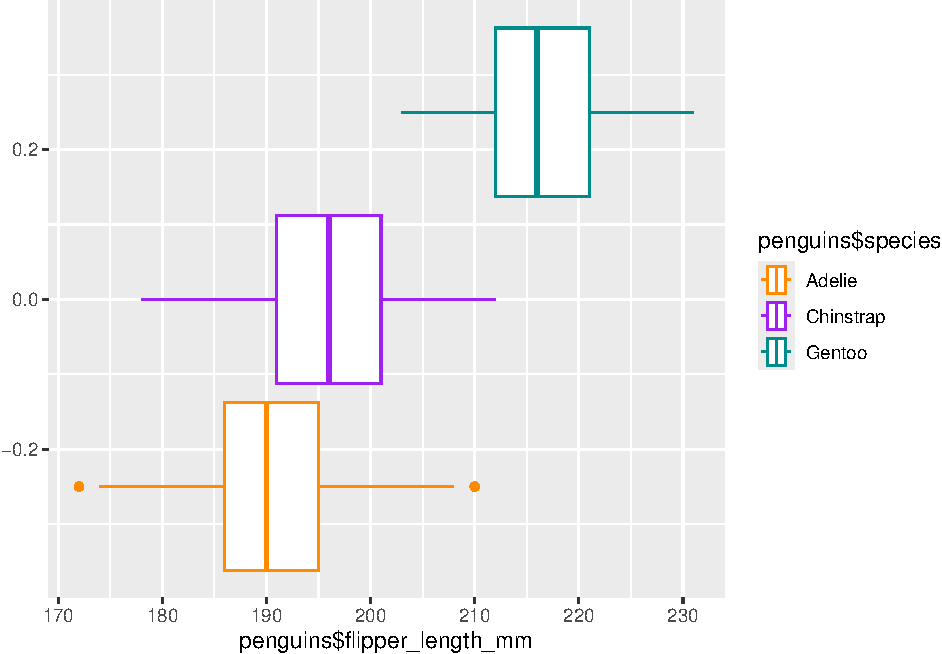
\includegraphics{es_files/figure-latex/unnamed-chunk-11-1.pdf}

\hypertarget{d-2}{%
\subsection{D}\label{d-2}}

Compute the flipper length quartiles for the ``Gentoo'' penguins (Q1,
Q2, Q3).

\begin{Shaded}
\begin{Highlighting}[]
\NormalTok{gentoo \textless{}{-}}\StringTok{ }\NormalTok{penguins[penguins}\OperatorTok{$}\NormalTok{species }\OperatorTok{==}\StringTok{ "Gentoo"}\NormalTok{, ]}
\NormalTok{quartiles \textless{}{-}}\StringTok{ }\KeywordTok{quantile}\NormalTok{(}
\NormalTok{  gentoo}\OperatorTok{$}\NormalTok{flipper\_length\_mm,}
  \KeywordTok{c}\NormalTok{(}\FloatTok{0.25}\NormalTok{, }\FloatTok{0.5}\NormalTok{, }\FloatTok{0.75}\NormalTok{),}
  \DataTypeTok{na.rm =} \OtherTok{TRUE}
\NormalTok{)}
\NormalTok{quartiles}
\end{Highlighting}
\end{Shaded}

\begin{verbatim}
## 25% 50% 75% 
## 212 216 221
\end{verbatim}

\hypertarget{e-1}{%
\subsection{E}\label{e-1}}

Calculate the flipper length 40th percentile for the ``Adelie''
penguins.

\begin{Shaded}
\begin{Highlighting}[]
\NormalTok{adelie \textless{}{-}}\StringTok{ }\NormalTok{penguins[penguins}\OperatorTok{$}\NormalTok{species }\OperatorTok{==}\StringTok{ "Adelie"}\NormalTok{, ]}
\NormalTok{p40 \textless{}{-}}\StringTok{ }\KeywordTok{quantile}\NormalTok{(}
\NormalTok{  adelie}\OperatorTok{$}\NormalTok{flipper\_length\_mm,}
  \FloatTok{0.4}\NormalTok{,}
  \DataTypeTok{na.rm =} \OtherTok{TRUE}
\NormalTok{)}
\NormalTok{p40}
\end{Highlighting}
\end{Shaded}

\begin{verbatim}
## 40% 
## 189
\end{verbatim}

\hypertarget{exercise-4---multiple-boxplots-from-scratch}{%
\section{Exercise 4 - Multiple boxplots from
scratch}\label{exercise-4---multiple-boxplots-from-scratch}}

\hypertarget{a-3}{%
\subsection{A}\label{a-3}}

Generate random data with some structure, and create one data set for
each day of the week (hint: use the for() cycle, data should have 7
columns). At the end you should obtain a matrix with N rows (N = number
of random number to generate each time) and 7 columns (one for each day
of the week).

\begin{Shaded}
\begin{Highlighting}[]
\KeywordTok{set.seed}\NormalTok{(}\DecValTok{123}\NormalTok{)}
\NormalTok{n \textless{}{-}}\StringTok{ }\DecValTok{10}
\NormalTok{days \textless{}{-}}\StringTok{ }\KeywordTok{c}\NormalTok{(}
  \StringTok{"Monday"}\NormalTok{,}
  \StringTok{"Tuesday"}\NormalTok{,}
  \StringTok{"Wednesday"}\NormalTok{,}
  \StringTok{"Thursday"}\NormalTok{,}
  \StringTok{"Friday"}\NormalTok{,}
  \StringTok{"Saturday"}\NormalTok{,}
  \StringTok{"Sunday"}
\NormalTok{)}
\NormalTok{data \textless{}{-}}\StringTok{ }\KeywordTok{matrix}\NormalTok{(}\DataTypeTok{nrow =}\NormalTok{ n, }\DataTypeTok{ncol =} \DecValTok{7}\NormalTok{)}

\ControlFlowTok{for}\NormalTok{ (i }\ControlFlowTok{in} \DecValTok{1}\OperatorTok{:}\DecValTok{7}\NormalTok{) \{}
\NormalTok{  data[, i] \textless{}{-}}\StringTok{ }\KeywordTok{round}\NormalTok{(}\KeywordTok{runif}\NormalTok{(n, }\DataTypeTok{min =} \DecValTok{0}\NormalTok{, }\DataTypeTok{max =} \DecValTok{100}\NormalTok{), }\DecValTok{0}\NormalTok{)}
\NormalTok{\}}

\NormalTok{df \textless{}{-}}\StringTok{ }\KeywordTok{data.frame}\NormalTok{(data)}
\KeywordTok{colnames}\NormalTok{(df) \textless{}{-}}\StringTok{ }\NormalTok{days}
\NormalTok{df}
\end{Highlighting}
\end{Shaded}

\begin{verbatim}
##    Monday Tuesday Wednesday Thursday Friday Saturday Sunday
## 1      29      96        89       96     14        5     67
## 2      79      45        69       90     41       44      9
## 3      41      68        64       69     41       80     38
## 4      88      57        99       80     37       12     27
## 5      94      10        66        2     15       56     81
## 6       5      90        71       48     14       21     45
## 7      53      25        54       76     23       13     81
## 8      89       4        59       22     47       75     81
## 9      55      33        29       32     27       90     79
## 10     46      95        15       23     86       37     44
\end{verbatim}

\hypertarget{b-3}{%
\subsection{B}\label{b-3}}

Go from a wide to a long data format. You should create a data.frame
object with exactly two columns. One contains the values created in A.,
the other contains the corresponding day of the week.

\begin{Shaded}
\begin{Highlighting}[]
\NormalTok{df\_long \textless{}{-}}\StringTok{ }\KeywordTok{data.frame}\NormalTok{(}
  \StringTok{"Day"}\NormalTok{ =}\StringTok{ }\KeywordTok{rep}\NormalTok{(days, }\DataTypeTok{each =}\NormalTok{ n),}
  \StringTok{"Value"}\NormalTok{ =}\StringTok{ }\KeywordTok{c}\NormalTok{(}
\NormalTok{    df}\OperatorTok{$}\NormalTok{Monday,}
\NormalTok{    df}\OperatorTok{$}\NormalTok{Tuesday,}
\NormalTok{    df}\OperatorTok{$}\NormalTok{Wednesday,}
\NormalTok{    df}\OperatorTok{$}\NormalTok{Thursday,}
\NormalTok{    df}\OperatorTok{$}\NormalTok{Friday,}
\NormalTok{    df}\OperatorTok{$}\NormalTok{Saturday,}
\NormalTok{    df}\OperatorTok{$}\NormalTok{Sunday}
\NormalTok{  )}
\NormalTok{)}
\NormalTok{df\_long}
\end{Highlighting}
\end{Shaded}

\begin{verbatim}
##          Day Value
## 1     Monday    29
## 2     Monday    79
## 3     Monday    41
## 4     Monday    88
## 5     Monday    94
## 6     Monday     5
## 7     Monday    53
## 8     Monday    89
## 9     Monday    55
## 10    Monday    46
## 11   Tuesday    96
## 12   Tuesday    45
## 13   Tuesday    68
## 14   Tuesday    57
## 15   Tuesday    10
## 16   Tuesday    90
## 17   Tuesday    25
## 18   Tuesday     4
## 19   Tuesday    33
## 20   Tuesday    95
## 21 Wednesday    89
## 22 Wednesday    69
## 23 Wednesday    64
## 24 Wednesday    99
## 25 Wednesday    66
## 26 Wednesday    71
## 27 Wednesday    54
## 28 Wednesday    59
## 29 Wednesday    29
## 30 Wednesday    15
## 31  Thursday    96
## 32  Thursday    90
## 33  Thursday    69
## 34  Thursday    80
## 35  Thursday     2
## 36  Thursday    48
## 37  Thursday    76
## 38  Thursday    22
## 39  Thursday    32
## 40  Thursday    23
## 41    Friday    14
## 42    Friday    41
## 43    Friday    41
## 44    Friday    37
## 45    Friday    15
## 46    Friday    14
## 47    Friday    23
## 48    Friday    47
## 49    Friday    27
## 50    Friday    86
## 51  Saturday     5
## 52  Saturday    44
## 53  Saturday    80
## 54  Saturday    12
## 55  Saturday    56
## 56  Saturday    21
## 57  Saturday    13
## 58  Saturday    75
## 59  Saturday    90
## 60  Saturday    37
## 61    Sunday    67
## 62    Sunday     9
## 63    Sunday    38
## 64    Sunday    27
## 65    Sunday    81
## 66    Sunday    45
## 67    Sunday    81
## 68    Sunday    81
## 69    Sunday    79
## 70    Sunday    44
\end{verbatim}

\hypertarget{c-3}{%
\subsection{C}\label{c-3}}

Plot the seven boxplots (one for each day of the week) in one graph,
horizontally oriented (hint: coord\_flip() function translates the axes,
the ``limits'' argument of scale\_x\_discrete() allows you to reorder
the axis labels).

\begin{Shaded}
\begin{Highlighting}[]
\KeywordTok{ggplot}\NormalTok{(}
\NormalTok{  df\_long,}
  \KeywordTok{aes}\NormalTok{(}
    \DataTypeTok{x =}\NormalTok{ Day,}
    \DataTypeTok{y =}\NormalTok{ Value,}
    \DataTypeTok{color =}\NormalTok{ Day}
\NormalTok{  )}
\NormalTok{) }\OperatorTok{+}
\StringTok{  }\KeywordTok{scale\_color\_manual}\NormalTok{(}\DataTypeTok{values =} \KeywordTok{rainbow}\NormalTok{(}\DecValTok{7}\NormalTok{)) }\OperatorTok{+}
\StringTok{  }\KeywordTok{scale\_x\_discrete}\NormalTok{(}\DataTypeTok{limits =} \KeywordTok{rev}\NormalTok{(days)) }\OperatorTok{+}
\StringTok{  }\KeywordTok{geom\_boxplot}\NormalTok{() }\OperatorTok{+}
\StringTok{  }\KeywordTok{coord\_flip}\NormalTok{() }\OperatorTok{+}
\StringTok{  }\KeywordTok{labs}\NormalTok{(}
    \DataTypeTok{title =} \StringTok{"Random values by day of the week"}\NormalTok{,}
    \DataTypeTok{x =} \StringTok{"Day of the week"}\NormalTok{,}
    \DataTypeTok{y =} \StringTok{"Random value"}\NormalTok{,}
    \DataTypeTok{color =} \StringTok{"Day of the week"}
\NormalTok{  )}
\end{Highlighting}
\end{Shaded}

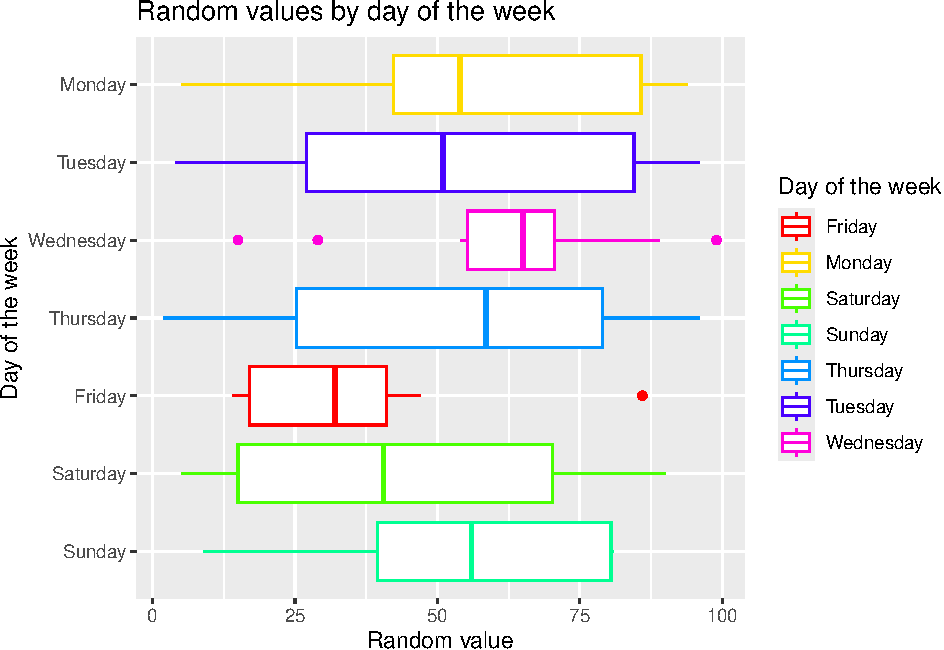
\includegraphics{es_files/figure-latex/unnamed-chunk-16-1.pdf}

\hypertarget{exercise-5---exploratory-analysis-of-data}{%
\section{Exercise 5 - Exploratory analysis of
data}\label{exercise-5---exploratory-analysis-of-data}}

Penguins dataset does not contain their weights and flipper lengths
only. Many other variables are available. Let's explore it a little
more:

\hypertarget{a-4}{%
\subsection{A}\label{a-4}}

How many islands are there? And how many penguins are present in each
isle? Are the 3 species of penguins living together? (hint: use the
table() function).

\begin{Shaded}
\begin{Highlighting}[]
\KeywordTok{cat}\NormalTok{(}\StringTok{"The number of islands is: "}\NormalTok{, }\KeywordTok{length}\NormalTok{(}\KeywordTok{unique}\NormalTok{(penguins}\OperatorTok{$}\NormalTok{island)), }\StringTok{"}\CharTok{\textbackslash{}n}\StringTok{"}\NormalTok{)}
\end{Highlighting}
\end{Shaded}

\begin{verbatim}
## The number of islands is:  3
\end{verbatim}

\begin{Shaded}
\begin{Highlighting}[]
\KeywordTok{table}\NormalTok{(penguins}\OperatorTok{$}\NormalTok{island)}
\end{Highlighting}
\end{Shaded}

\begin{verbatim}
## 
##    Biscoe     Dream Torgersen 
##       168       124        52
\end{verbatim}

\begin{Shaded}
\begin{Highlighting}[]
\KeywordTok{table}\NormalTok{(penguins}\OperatorTok{$}\NormalTok{island, penguins}\OperatorTok{$}\NormalTok{species)}
\end{Highlighting}
\end{Shaded}

\begin{verbatim}
##            
##             Adelie Chinstrap Gentoo
##   Biscoe        44         0    124
##   Dream         56        68      0
##   Torgersen     52         0      0
\end{verbatim}

\hypertarget{b-4}{%
\subsection{B}\label{b-4}}

Try to use the geom\_bar() or geom\_col() functions to graphically
represent the population of each island, colored by species (hint:
islands in the x-axis, number of penguins in the y-axis).

\begin{Shaded}
\begin{Highlighting}[]
\KeywordTok{ggplot}\NormalTok{(}
\NormalTok{  penguins,}
  \KeywordTok{aes}\NormalTok{(}
    \DataTypeTok{x =}\NormalTok{ island,}
    \DataTypeTok{fill =}\NormalTok{ species}
\NormalTok{  )}
\NormalTok{) }\OperatorTok{+}
\StringTok{  }\KeywordTok{geom\_bar}\NormalTok{() }\OperatorTok{+}
\StringTok{  }\KeywordTok{scale\_fill\_manual}\NormalTok{(}\DataTypeTok{values =} \KeywordTok{c}\NormalTok{(}\StringTok{"darkorange"}\NormalTok{, }\StringTok{"purple"}\NormalTok{, }\StringTok{"cyan4"}\NormalTok{)) }\OperatorTok{+}
\StringTok{  }\KeywordTok{labs}\NormalTok{(}
    \DataTypeTok{title =} \StringTok{"Penguins population by island"}\NormalTok{,}
    \DataTypeTok{x =} \StringTok{"Island"}\NormalTok{,}
    \DataTypeTok{y =} \StringTok{"Number of penguins"}\NormalTok{,}
    \DataTypeTok{fill =} \StringTok{"Species"}
\NormalTok{  )}
\end{Highlighting}
\end{Shaded}

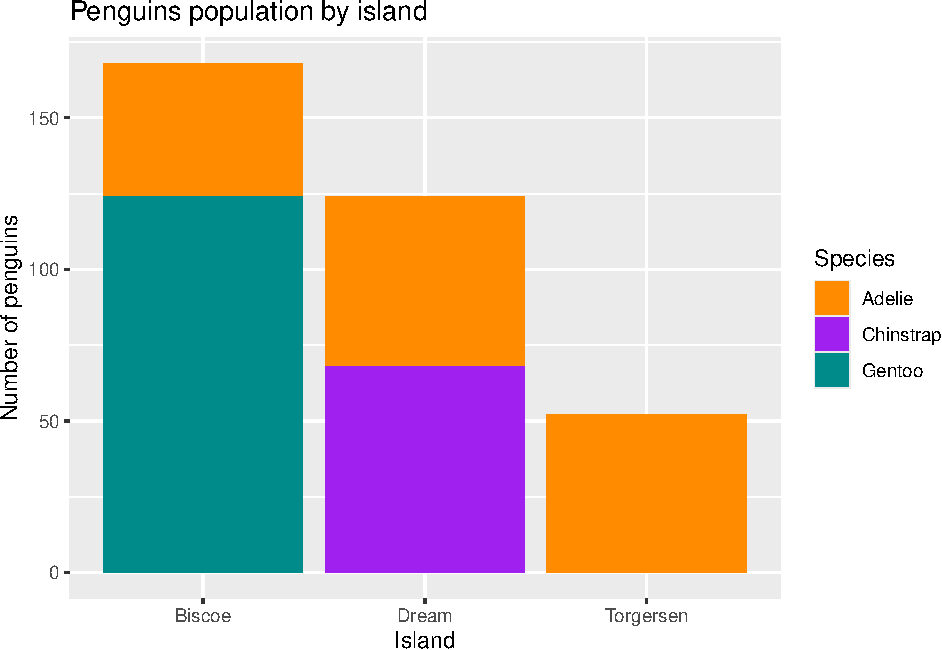
\includegraphics{es_files/figure-latex/unnamed-chunk-18-1.pdf}

\hypertarget{c-4}{%
\subsection{C}\label{c-4}}

Use a scatter plot to represent flipper length vs.~body mass. Color the
point according to the ``sex'' variable. Try to use facets to see if
there are differences across species (hint: use
facet\_grid(\textasciitilde{} species) function to add facets for
species).

\begin{Shaded}
\begin{Highlighting}[]
\KeywordTok{ggplot}\NormalTok{(}
\NormalTok{  penguins,}
  \KeywordTok{aes}\NormalTok{(}
    \DataTypeTok{x =}\NormalTok{ penguins}\OperatorTok{$}\NormalTok{flipper\_length\_mm,}
    \DataTypeTok{y =}\NormalTok{ penguins}\OperatorTok{$}\NormalTok{body\_mass\_g,}
    \DataTypeTok{color =}\NormalTok{ penguins}\OperatorTok{$}\NormalTok{sex}
\NormalTok{  )}
\NormalTok{) }\OperatorTok{+}
\StringTok{  }\KeywordTok{geom\_point}\NormalTok{() }\OperatorTok{+}
\StringTok{  }\KeywordTok{facet\_grid}\NormalTok{(}\OperatorTok{\textasciitilde{}}\NormalTok{species) }\OperatorTok{+}
\StringTok{  }\KeywordTok{scale\_color\_manual}\NormalTok{(}\DataTypeTok{values =} \KeywordTok{c}\NormalTok{(}\StringTok{"blue"}\NormalTok{, }\StringTok{"magenta"}\NormalTok{)) }\OperatorTok{+}
\StringTok{  }\KeywordTok{labs}\NormalTok{(}
    \DataTypeTok{title =} \StringTok{"Flipper length vs. body mass"}\NormalTok{,}
    \DataTypeTok{x =} \StringTok{"Flipper length (mm)"}\NormalTok{,}
    \DataTypeTok{y =} \StringTok{"Body mass (g)"}\NormalTok{,}
    \DataTypeTok{color =} \StringTok{"Sex"}
\NormalTok{  )}
\end{Highlighting}
\end{Shaded}

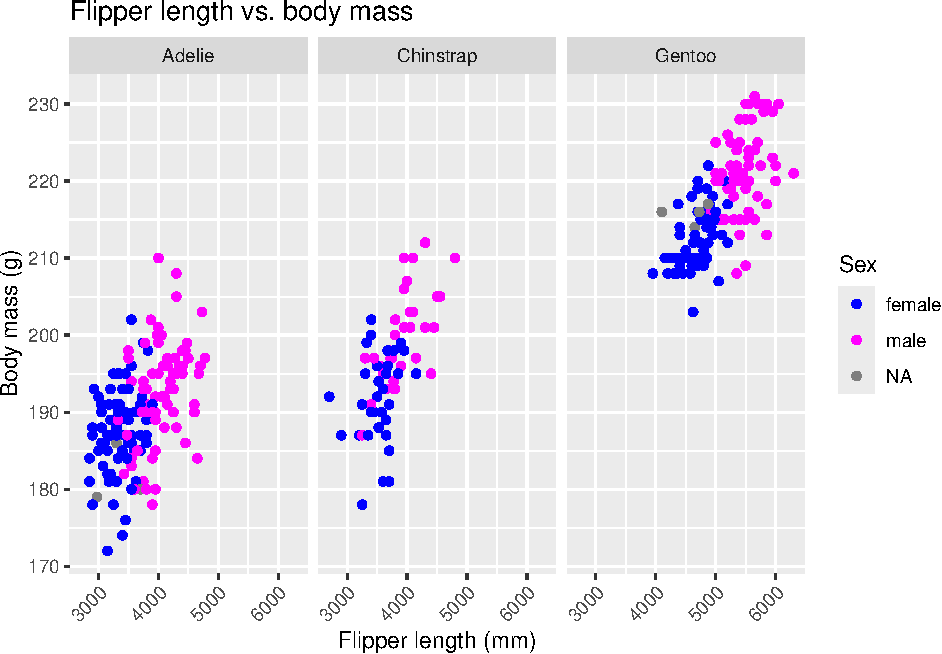
\includegraphics{es_files/figure-latex/unnamed-chunk-19-1.pdf}

\hypertarget{d-3}{%
\subsection{D}\label{d-3}}

The numeric variables shows some interesting relationships. Are they
correlated? Use the cor() and the corrplot() functions to study
correlations between numeric variables (hint: try to google corrplot()
to see which package you have to install to use it).

\begin{Shaded}
\begin{Highlighting}[]
\KeywordTok{library}\NormalTok{(corrplot)}
\NormalTok{correlation \textless{}{-}}\StringTok{ }\KeywordTok{cor}\NormalTok{(penguins[, }\KeywordTok{c}\NormalTok{(}\DecValTok{3}\OperatorTok{:}\DecValTok{6}\NormalTok{, }\DecValTok{8}\NormalTok{)], }\DataTypeTok{use =} \StringTok{"complete.obs"}\NormalTok{)}
\KeywordTok{corrplot}\NormalTok{(correlation, }\DataTypeTok{method =} \StringTok{"number"}\NormalTok{)}
\end{Highlighting}
\end{Shaded}

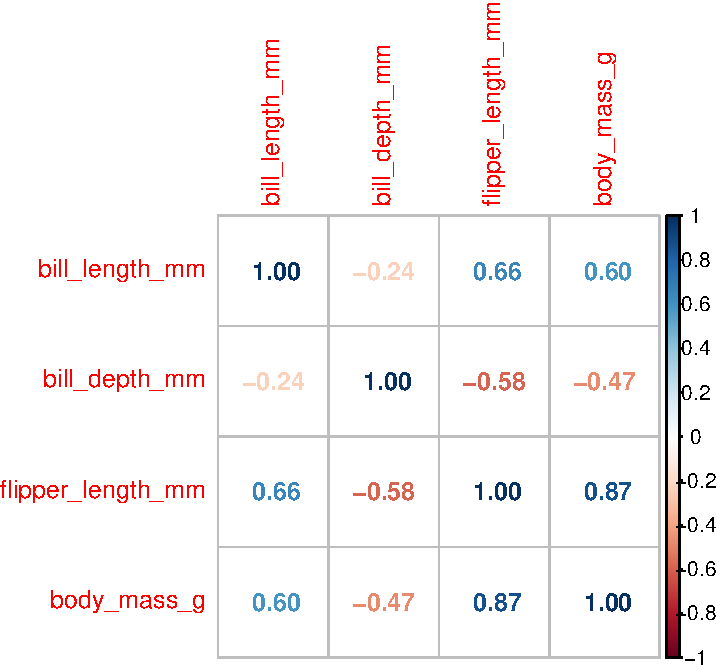
\includegraphics{es_files/figure-latex/unnamed-chunk-20-1.pdf}

\begin{Shaded}
\begin{Highlighting}[]
\KeywordTok{corrplot}\NormalTok{(correlation, }\DataTypeTok{method =} \StringTok{"color"}\NormalTok{)}
\end{Highlighting}
\end{Shaded}

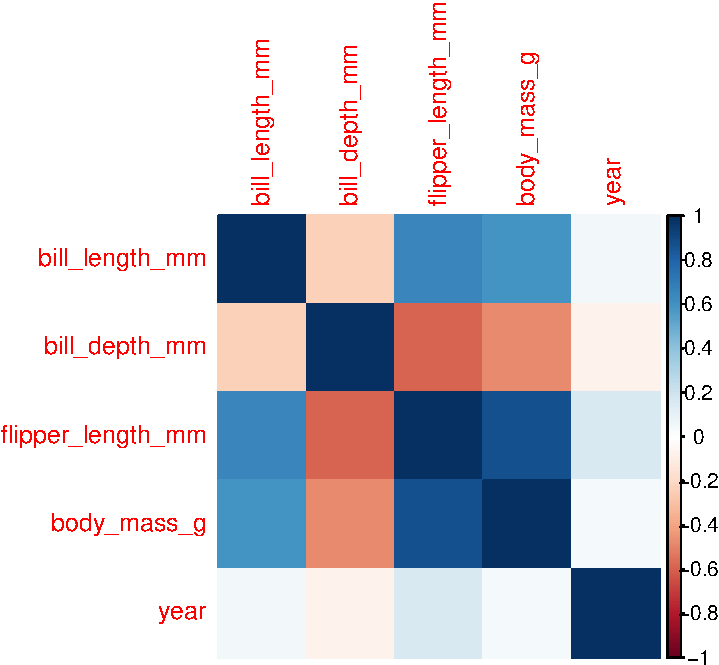
\includegraphics{es_files/figure-latex/unnamed-chunk-21-1.pdf}

\begin{Shaded}
\begin{Highlighting}[]
\KeywordTok{corrplot}\NormalTok{(correlation)}
\end{Highlighting}
\end{Shaded}

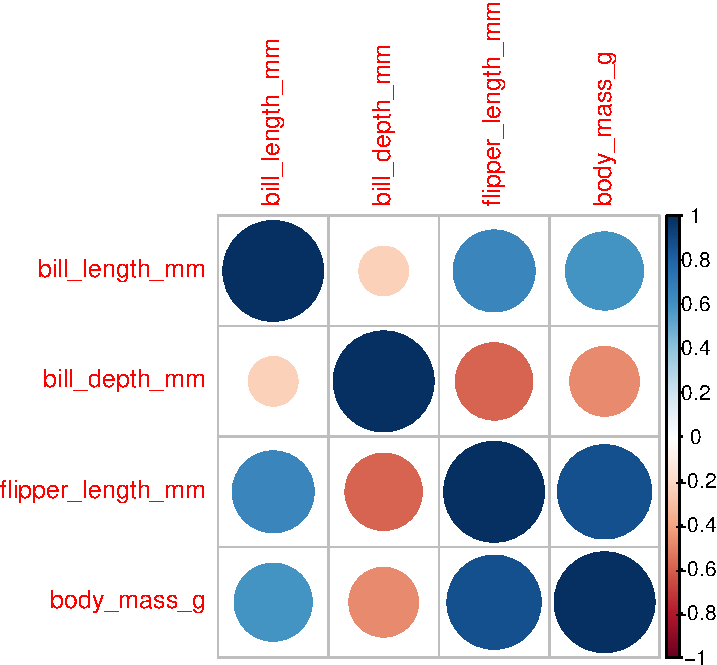
\includegraphics{es_files/figure-latex/unnamed-chunk-22-1.pdf}

\begin{Shaded}
\begin{Highlighting}[]
\KeywordTok{corrplot}\NormalTok{(correlation, }\DataTypeTok{order =} \StringTok{"AOE"}\NormalTok{)}
\end{Highlighting}
\end{Shaded}

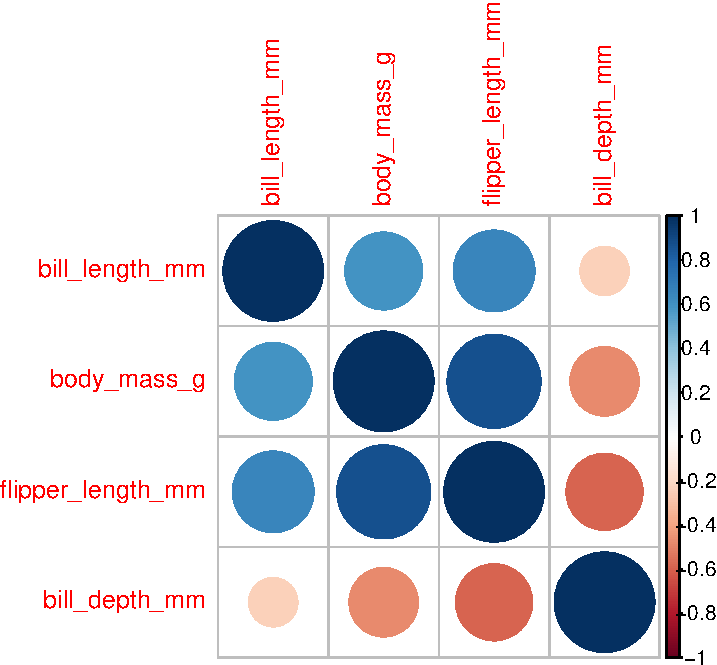
\includegraphics{es_files/figure-latex/unnamed-chunk-23-1.pdf}

\hypertarget{e-2}{%
\subsection{E}\label{e-2}}

Choose a pair of numeric variables, compute the correlation between them
without using the cor() function (hint: remember the formula).

\begin{Shaded}
\begin{Highlighting}[]
\NormalTok{x \textless{}{-}}\StringTok{ }\NormalTok{penguins}\OperatorTok{$}\NormalTok{flipper\_length\_mm}
\NormalTok{y \textless{}{-}}\StringTok{ }\NormalTok{penguins}\OperatorTok{$}\NormalTok{body\_mass\_g}

\NormalTok{n \textless{}{-}}\StringTok{ }\KeywordTok{length}\NormalTok{(x)}
\NormalTok{mean\_x \textless{}{-}}\StringTok{ }\KeywordTok{mean}\NormalTok{(x, }\DataTypeTok{na.rm =} \OtherTok{TRUE}\NormalTok{)}
\NormalTok{mean\_y \textless{}{-}}\StringTok{ }\KeywordTok{mean}\NormalTok{(y, }\DataTypeTok{na.rm =} \OtherTok{TRUE}\NormalTok{)}

\NormalTok{covariance \textless{}{-}}\StringTok{ }\KeywordTok{sum}\NormalTok{((x }\OperatorTok{{-}}\StringTok{ }\NormalTok{mean\_x) }\OperatorTok{*}\StringTok{ }\NormalTok{(y }\OperatorTok{{-}}\StringTok{ }\NormalTok{mean\_y), }\DataTypeTok{na.rm =} \OtherTok{TRUE}\NormalTok{) }\OperatorTok{/}\StringTok{ }\NormalTok{(n }\OperatorTok{{-}}\StringTok{ }\DecValTok{1}\NormalTok{)}
\NormalTok{sd\_x \textless{}{-}}\StringTok{ }\KeywordTok{sqrt}\NormalTok{(}\KeywordTok{sum}\NormalTok{((x }\OperatorTok{{-}}\StringTok{ }\NormalTok{mean\_x)}\OperatorTok{\^{}}\DecValTok{2}\NormalTok{, }\DataTypeTok{na.rm =} \OtherTok{TRUE}\NormalTok{) }\OperatorTok{/}\StringTok{ }\NormalTok{(n }\OperatorTok{{-}}\StringTok{ }\DecValTok{1}\NormalTok{))}
\NormalTok{sd\_y \textless{}{-}}\StringTok{ }\KeywordTok{sqrt}\NormalTok{(}\KeywordTok{sum}\NormalTok{((y }\OperatorTok{{-}}\StringTok{ }\NormalTok{mean\_y)}\OperatorTok{\^{}}\DecValTok{2}\NormalTok{, }\DataTypeTok{na.rm =} \OtherTok{TRUE}\NormalTok{) }\OperatorTok{/}\StringTok{ }\NormalTok{(n }\OperatorTok{{-}}\StringTok{ }\DecValTok{1}\NormalTok{))}

\NormalTok{correlation \textless{}{-}}\StringTok{ }\NormalTok{covariance }\OperatorTok{/}\StringTok{ }\NormalTok{(sd\_x }\OperatorTok{*}\StringTok{ }\NormalTok{sd\_y)}
\KeywordTok{cat}\NormalTok{(}
  \StringTok{"The correlation between flipper length and body mass is: "}\NormalTok{,}
\NormalTok{  correlation, }\StringTok{"}\CharTok{\textbackslash{}n}\StringTok{"}
\NormalTok{)}
\end{Highlighting}
\end{Shaded}

\begin{verbatim}
## The correlation between flipper length and body mass is:  0.8712018
\end{verbatim}

\hypertarget{f}{%
\subsection{F}\label{f}}

Plot the scatter plot for bill length vs.~bill depth. Color the points
by species. Use the function geom\_smooth(formula = ``y
\textasciitilde{} x'') to add a line to represent the linear
relationship between the two variables. Then, again, use
geom\_smooth(formula = ``y \textasciitilde{} x'') colored by species.
What are you noticing?

\begin{Shaded}
\begin{Highlighting}[]
\KeywordTok{ggplot}\NormalTok{(}
\NormalTok{  penguins,}
  \KeywordTok{aes}\NormalTok{(}
    \DataTypeTok{x =}\NormalTok{ penguins}\OperatorTok{$}\NormalTok{bill\_length\_mm,}
    \DataTypeTok{y =}\NormalTok{ penguins}\OperatorTok{$}\NormalTok{bill\_depth\_mm,}
    \DataTypeTok{color =}\NormalTok{ penguins}\OperatorTok{$}\NormalTok{species}
\NormalTok{  )}
\NormalTok{) }\OperatorTok{+}
\StringTok{  }\KeywordTok{geom\_point}\NormalTok{() }\OperatorTok{+}
\StringTok{  }\KeywordTok{geom\_smooth}\NormalTok{(}
    \DataTypeTok{formula =} \StringTok{"y \textasciitilde{} x"}\NormalTok{,}
    \DataTypeTok{method =} \StringTok{"lm"}\NormalTok{,}
    \KeywordTok{aes}\NormalTok{(}\DataTypeTok{color =}\NormalTok{ penguins}\OperatorTok{$}\NormalTok{species),}
    \DataTypeTok{se =} \OtherTok{FALSE}
\NormalTok{  ) }\OperatorTok{+}
\StringTok{  }\KeywordTok{scale\_color\_manual}\NormalTok{(}\DataTypeTok{values =} \KeywordTok{c}\NormalTok{(}\StringTok{"darkorange"}\NormalTok{, }\StringTok{"purple"}\NormalTok{, }\StringTok{"cyan4"}\NormalTok{)) }\OperatorTok{+}
\StringTok{  }\KeywordTok{labs}\NormalTok{(}
    \DataTypeTok{title =} \StringTok{"Bill length vs. bill depth"}\NormalTok{,}
    \DataTypeTok{x =} \StringTok{"Bill length (mm)"}\NormalTok{,}
    \DataTypeTok{y =} \StringTok{"Bill depth (mm)"}\NormalTok{,}
    \DataTypeTok{color =} \StringTok{"Species"}
\NormalTok{  )}
\end{Highlighting}
\end{Shaded}

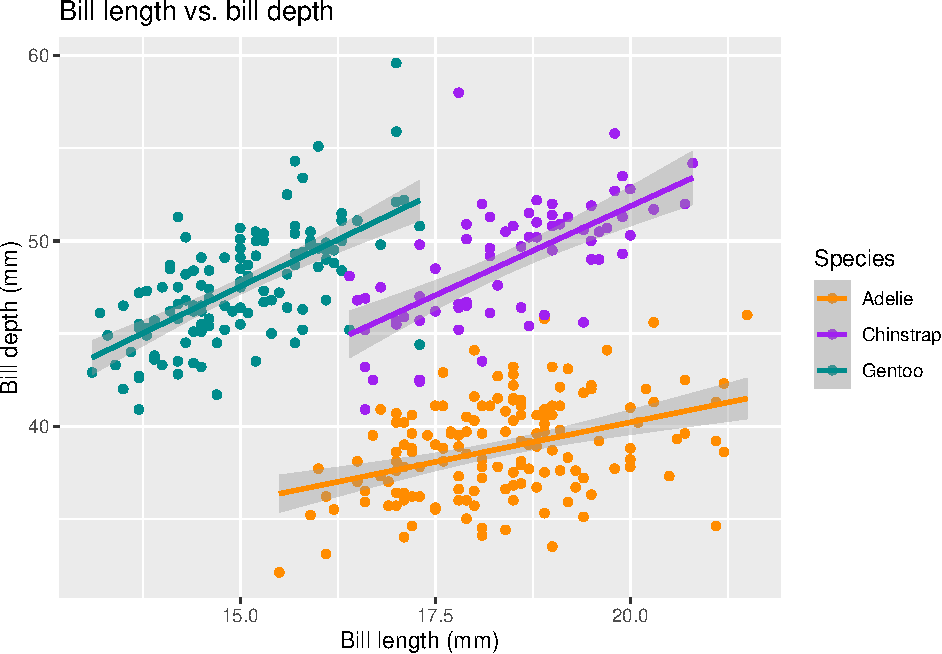
\includegraphics{es_files/figure-latex/unnamed-chunk-25-1.pdf}

\end{document}
